\documentclass[10pt]{beamer}

\usetheme[progressbar=foot]{metropolis}
\usepackage{appendixnumberbeamer}

\usepackage{booktabs}
\usepackage[scale=2]{ccicons}

\usepackage{pgfplots}
\usepgfplotslibrary{dateplot}
\pgfplotsset{compat=1.18} 

\usepackage{xspace}
\usepackage{xcolor}

\DeclareMathOperator{\stdev}{stdev}
\DeclareMathOperator{\var}{var}
\DeclareMathOperator{\cov}{cov}
\DeclareMathOperator{\corr}{corr}
\DeclareMathOperator{\prob}{prob}
\DeclareMathOperator{\n}{n}
\DeclareMathOperator{\N}{N}
\DeclareMathOperator{\Cov}{Cov}

\newcommand{\hlf}{\frac{1}{2}}
\newcommand{\bi}{\begin{itemize}}
\newcommand{\ei}{\end{itemize}}
\newcommand{\im}{\item}
\newcommand{\D}{\mathrm{d}}
\newcommand{\E}{\mathrm{e}}
\newcommand{\mye}{\ensuremath{\mathsf{E}}}
\newcommand{\myreal}{\ensuremath{\mathbb{R}}}
\newcommand{\bq}{\begin{equation}}
\newcommand{\eq}{\end{equation}}
\newcommand{\eqdef}{\;\buildrel \text{d{}ef}\over = \;}
\newcommand{\xstar}{\buildrel *\over X}
\newcommand{\pmax}{p^{\text{max}}}
\newcommand{\qmax}{q^{\text{max}}}
\newcommand{\bfr}{\begin{frame}}
\newcommand{\bfrp}{\begin{frame}[plain]}
\newcommand{\efr}{\end{frame}}
\newcommand{\F}{\mathcal{F}}
\newcommand{\FF}{\mathbb{F}}
\newcommand{\ve}{\varepsilon}
\newcommand{\lh}{\hat{\lambda}}
\definecolor{mycolor}{gray}{0.8}
\definecolor{mymaincolor}{rgb}{0.6862745098039216,0.9333333333333333,0.9333333333333333}
\newcommand{\alr}[1]{\textcolor{blue}{#1}}
\definecolor{LightCyan}{rgb}{0.88,1,1}
\newcommand{\yel}{\cellcolor{yellow}}
\newcommand{\blue}{\cellcolor{SkyBlue}}
\newcommand{\gr}{\cellcolor{SpringGreen}}
\newcommand{\pink}{\cellcolor{pink}}
\newcommand{\apr}{\cellcolor{Apricot}}
\newcommand{\tve}{\tilde{\varepsilon}}
\newcommand{\tw}{\tilde{w}}
\newcommand{\ttth}{\tilde{\theta}}
\newcommand{\te}{\tilde{e}}
\newcommand{\ts}{\tilde{s}}
\newcommand{\tx}{\tilde{x}}
\newcommand{\ty}{\tilde{y}}
\newcommand{\tv}{\tilde{v}}
\newcommand{\tp}{\tilde{p}}
\newcommand{\tF}{\tilde{F}}
\newcommand{\tf}{\tilde{f}}
\newcommand{\tZ}{\tilde{Z}}
\newcommand{\ow}{\overline{w}}
\newcommand{\tm}{\tilde{m}}
\newcommand{\tc}{\tilde{c}}
\newcommand{\tz}{\tilde{z}}
\newcommand{\tr}{\widetilde{R}}
\newcommand{\tR}{\widetilde{\mathbf{R}}}
\newcommand{\bms}{\begin{multline*}}
\newcommand{\ems}{\end{multline*}}
\newcommand{\bas}{\begin{align*}}
\newcommand{\eas}{\end{align*}}
\newcommand{\qr}{\mathbb{Q}}
\newcommand{\tX}{\tilde{X}}
\newcommand{\tY}{\tilde{Y}}

\setbeamertemplate{frame footer}{BUSI 521/ECON 505/ECON 505}

\title{Chapter 9: Dynamic Portfolio Choice}

\date{}
\author{Kerry Back\\ 
BUSI 521/ECON 505\\
Rice University}


\begin{document}

\maketitle

\bfr\frametitle{A Dynamic Decision Problem}
The problem is to choose Up or Down at each date to maximize the terminal reward.  The optimal sequence of decisions is Down-Up-Up.
\begin{center}
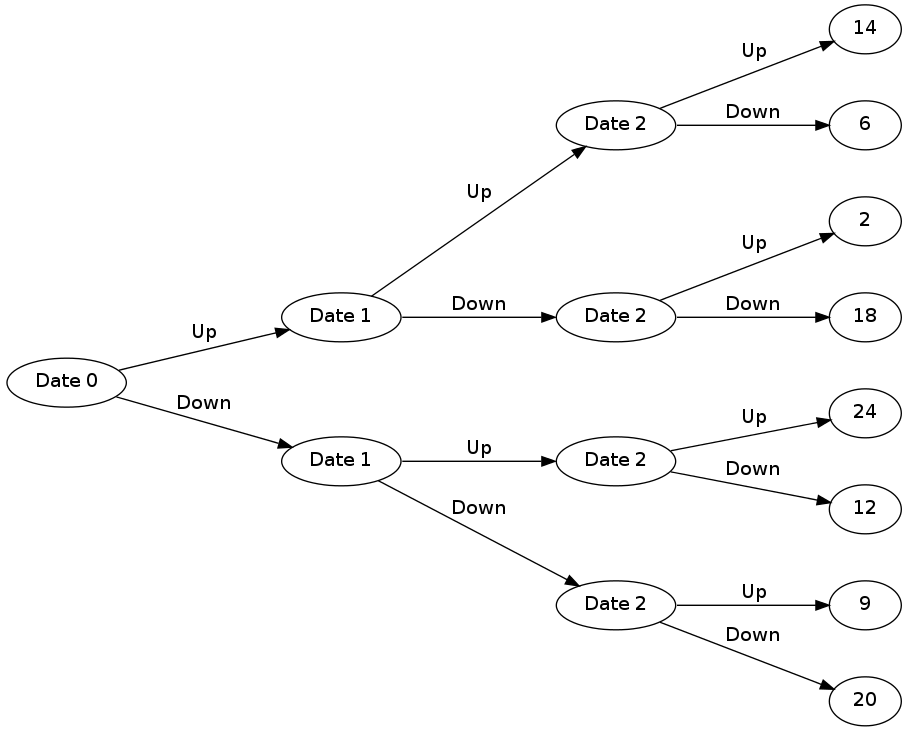
\includegraphics[scale=.2]{images/fig9_1.png}
\end{center}

\end{frame}

\bfr\frametitle{Value Function}
The value at each node is the maximum value that can be reached starting from that node.  The value is also the max of the Up and Down values at each node.
\begin{center}
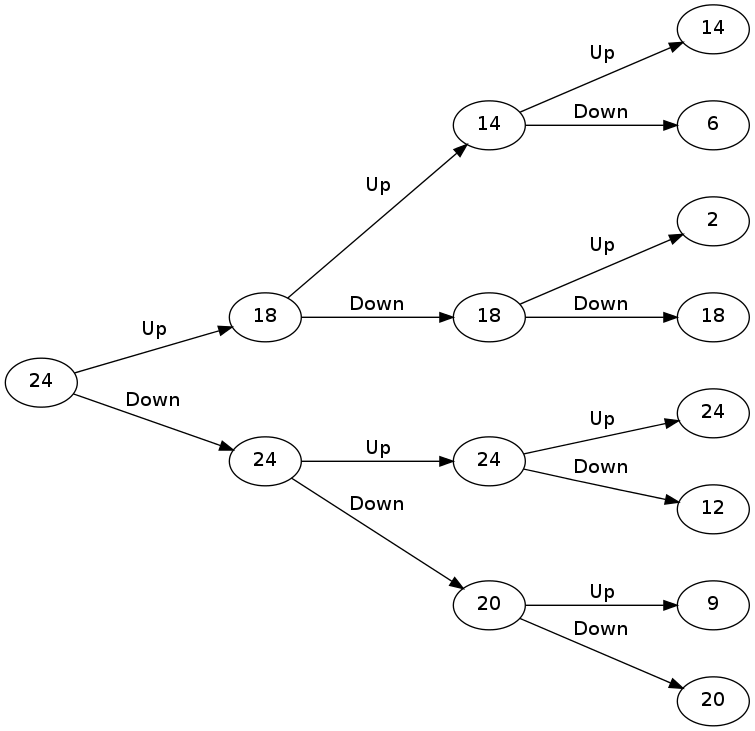
\includegraphics[scale=.2]{images/fig9_2.png}
\end{center}
\end{frame}


\bfr\frametitle{Bellman Equation}
\bi
\im Label the nodes at each date $t$ as $x=1,\ldots,2^t$, starting from the bottom.  Label the choice as $\pi=0$ for Up and $\pi=1$ for Down.  Then
$$x_{t+1} = 2x_t - \pi_t$$
\im Let $V_t(x)$ denote the value at node $x$ at date~$t$.  The value is the max of the Up and Down values, so
\bq\tag{$\star$}\label{eq1}
V_{t}(x) = \max_{\pi\in\{0,1\}} V_{t+1}(2x-\pi)
\eq
\im Equation \eqref{eq1} is called the Bellman equation.
\ei

\end{frame}

\bfr\frametitle{Intermediate Rewards}
\bi
\im Suppose there is a reward $u_t(x,\pi)$ at each date $t$, given the node $x$ at date $t$ and the decision $\pi$ taken at node $x$ at date $t$.  Suppose the objective is to maximize
$$\sum_{t=0}^2 u_{t}(x_t,\pi_{t}(x_t)) \;+\; u_3(x_3)\,,$$
\im 
Let $V_3(x) = u_3(x)$ and for $t<3$, define
\bq\label{eq2}\tag{$\star\star$}
V_{t}(x) = \max_{\pi\in\{0,1\}} \bigg\{u_{t}(x,\pi) + V_{t+1}(2x-\pi)\bigg\} 
\eq
\im $V_t$ is the value function and \eqref{eq2} is the Bellman equation with intermediate rewards.
\ei
\end{frame}

\bfr\frametitle{Dynamic Programming under Uncertainty}
For choice under uncertainty, the Bellman equation is
\bq\label{eq3}\tag{$\star\star\star$}
V_{t}( x) = \max_{\pi} \bigg\{u_{t}(x,\pi) + \mye[V_{t+1}(X_{t+1})\mid X_t=x]\bigg\}
\eq
Here $X_{t+1}$ denotes the random state (node) at date $t\!+\!1$, the distribution of which may depend on the decision~$\pi$ and the state~$x$ at date~$t$.  
\end{frame}

\bfr\frametitle{Markovian Model}
\bi
\im Assume $X$ is a stationary Markov process with values in $\myreal^k$.  This means that
\bi
\im the unconditional distribution of any finite set $(X_{t_1},X_{t_2},\ldots,X_{t_k})$ is the same as the distribution of $(X_{t_1+s},X_{t_2+s},\ldots,X_{t_k+s})$, for any $s$
\im the distribution of $X_{t+1}, X_{t+2}, \ldots$ conditional on all information at date $t$ is the same as the distribution conditional on $X_t$ only 
\ei
\im Assume the distribution of return vectors $R_{t+1}, R_{t+2}, \ldots$ and the distribution of labor income $Y_{t+1}, Y_{t+2}, \ldots$ conditional on all information at date $t$ is the same as the distribution conditional on $X_t$ only and are time homogeneous.
\im In other words, $X_t$ is a sufficient statistic for forecasting future values of $X$, $R$, and $Y$.
\ei
\end{frame}

 
\bfr\frametitle{Bellman Equation for Portfolio Choice}
\bi
\im Return vector $R_t \in \myreal^n$ includes risk-free return if it exists.
\im State variables are wealth $W$ and $X$.
\im Choice variables are consumption $c$ and portfolio $\pi$.  Require $\iota'\pi=1$.
\im Wealth evolves according to the intertemporal budget constraint:
$$W_{t+1} = (W_t-c)\pi'R_{t+1} + Y_{t+1}$$
\im Bellman equation: $V_t(x,w) = $
$$ \max_{c,\pi} \; \delta^t u(c) + \mye\left[\left. V_{t+1}\bigg(X_{t+1},(w-c)\pi'R_{t+1} + Y_{t+1}\bigg)\,\right|\, X_t=x\right]$$
\ei
\end{frame}

\bfr\frametitle{Discounting Back Only to Date $t$}
\bi
\im $V_t$ is the maximum expected sum of utilities at dates $t, t+1, \ldots$ measured in terms of date--0 utility, i.e., discounted to date~0.
\im The same expected sum measured in terms of date--$t$ utility is
$$J_t(x,w) = \delta^{-t}V_t(w,x)$$
\im Multiplying by $\delta^{-t}$ in the Bellman equation gives: $J_t(x,w) = $
$$ \max_{c,\pi} \; u(c) + \delta\mye\left[\left.   J_{t+1}\bigg(X_{t+1},Y(w-c)\pi'R_{t+1} + Y_{t+1}\bigg)\,\right|\, X_t=x\right]$$
\ei
\end{frame}

\bfr\frametitle{Infinite Horizon}
\bi
\im If there is an infinite horizon, then there is always an infinite number of periods remaining and $J$ does not depend on $t$.  
\im So the Bellman equation is: $J(x,w) = $
$$ \max_{c,\pi} \; u(c) + \delta\mye\left[\left.  J\bigg(X_{t+1},(w-c)\pi'R_{t+1} + Y_{t+1}]\bigg)\,\right|\, X_t=x\right]$$
\im Taking $t=0$, we can also write it as: $J(x,w) = $
$$ \max_{c,\pi} \; u(c) + \delta\mye\left[\left.  J\bigg(X_{1},(w-c)\pi'R_{1} + Y_1\bigg)\,\right|\, X_0=x\right]$$
\ei
\end{frame}

\section{Optimal Portfolio}
\subsection{}

\bfr\frametitle{Optimal Portfolio}
\bi
\im Consider the infinite horizon case for simplicity.
\im Let $c^*$ denote optimal consumption given $(x,w)$.  Then, the optimal portfolio $\pi^*$ solves
$$\max_\pi \; \mye\left[\left.J\bigg(X_{1},(w-c^*)\pi'R_{1} + Y_1\bigg)\,\right|\, X_0=x\right]$$
\im Compared to a single-period problem, the difference is that the objective function $J$ depends on $X_1$ in addition to depending on end-of-period wealth.
\im The optimal portfolio will usually, to some extent, hedge against adverse changes in $X$.
We discuss ``adverse changes'' further later.
\ei
\end{frame}

\bfr\frametitle{FOC for Optimal Portfolio}
\bi
\im Recall that we maximize over $\pi$ subject to $\iota'\pi=1$.  Use a subscript $w$ to denote a partial derivative with respect to wealth. 
\im FOC is
$$\mye\left[\left.J_w\bigg(X_{1},(w-c^*)\pi'R_{1}+ Y_1\bigg)R_{1}\,\right|\, X_0=x\right] = \lambda \iota$$
where $\lambda$ is the Lagrange multiplier for the constraint $\iota'\pi=1$.
\im Equivalently, $J_w/\lambda$ at the optimum is a single-period SDF (for some $\lambda$).
\ei
\end{frame}

\bfr\frametitle{Envelope Condition}
\bi
\im Consider the infinite horizon case for simplicity.

\im Let $c^*(x,w)$, $\pi^*(x,w)$ achieve the max in the Bellman equation.  
\im The envelope theorem implies that
$$J_w(x,w) = u'(c^*(x,w))$$
\im This is called the envelope condition: the marginal value of wealth equals the marginal utility of consumption at the optimum.
\ei
\end{frame}

\bfr\frametitle{SDF Process}
\bi
\im Recall the Euler equation:
$$\frac{\delta^t u'(C_t)}{u'(C_0)}$$
is an SDF process, where $C$ denotes optimal consumption.
\im In the Markovian model, the envelope condition and Euler equation imply
$$\frac{\delta^t J_w(X_t,W_t)}{J_w(X_0,W_0)}$$
is an SDF process, where $W$ denotes optimal wealth.
\ei
\end{frame}

\section{CRRA Utility}
\subsection{}

\bfr\frametitle{CRRA Utility}
\bi
\im Assume there is no labor income $Y$.  If $u$ is CRRA with risk aversion $\rho$, then $V$ and $J$ are CRRA in wealth $w$ with the same risk aversion $\rho$.
\im With an infinite horizon,
\bi
\im Log utility implies 
$$J(x,w) = f(x) + \gamma \log w$$ for a function $f$ and constant $\gamma$.
\im Power utility implies 
$$J(x,w) = f(x) \cdot \frac{1}{1-\rho}w^{1-\rho}$$
for a function $f$.
\ei 
\ei
\end{frame}

\bfr\frametitle{Example: Maximize Expected Log of Terminal Wealth}
\bi
\im Suppose the objective is to maximize $\mye[\log W_T]$ with no consumption prior to $T$.  Suppose there is no labor income $Y$.
\im Intertemporal budget constraint implies
$$W_{t+1} = W_t\pi_t'R_{t+1}$$
\im Bellman equation is
 $$V_t(x,w) = \max_{\pi} \; \mye\left[\left. V_{t+1}\bigg(X_{t+1},w\pi'R_{t+1}\bigg)\,\right|\, X_t=x\right]$$
 \im Terminal condition is $V_T(x,w) = \log w$.
 \ei
\end{frame}

\bfr\frametitle{Value Function and Optimal Portfolio}
\bi
\im Claim that $V_t(x,w) = f_t(x) + \log w$ for functions $f_t$.
 \im Clearly true for $t=T$ (with $f_T=0$)  Suppose it is true at $t+1, t+2, \ldots, T$ for some date $t$.  Then, the Bellman equation implies
 \begin{align*}
 V_t(x,w) &= \max_{\pi} \; \mye\left[\left. f_{t+1}(X_{t+1}) +  \log ( w\pi'R_{t+1})\,\right|\, X_t=x\right]\\
 &= \log w + \max_{\pi} \; \mye\left[\left. f_{t+1}(X_{t+1}) +  \log ( \pi'R_{t+1})\,\right|\, X_t=x\right]\\
 & \eqdef \log w + f_t(x)
 \end{align*}
 \im The maximization in $\pi$ is equivalent to
 $$\max_{\pi} \; \mye\left[\left. \log ( \pi'R_{t+1})\,\right|\, X_t=x\right]$$
 \im A log investor cares only about the distribution of the return $\pi'R_{t+1}$.  He does not hedge against adverse changes in $X$.
\ei
\end{frame}

\bfr\frametitle{Marginal Value of Wealth}
\bi
\im The ``no hedging'' result for log utility is due to the fact that $J_w$ does not depend on $x$:
$$J = f_t(x) + \gamma_t \log w \quad \Rightarrow \quad J_w = \frac{\gamma_t}{w}$$
\im Thus, the cross-partial $J_{wx_i} = 0$ for $i=1,\ldots, k$ for log utility.
This is a borderline case. 
\bi
\im For CRRA utility with $\rho<1$,  $J_{wx_i}$ has the same sign as $J_{x_i}$.
\im For CRRA utility with $\rho>1$, $J_{wx_i}$ has the opposite sign of $J_{x_i}$.
\ei
\im These facts affect hedging demands and risk premia (when investors have CRRA utility).
\ei
\end{frame}

\bfr\frametitle{Interpreting the Cross-Partial}
\bi
\im Example: Suppose $J_{x_i}>0$.  Then an increase in $x_i$ indicates ``good times''.  The investor gets higher expected future value when $x_i$ is higher.
\bi
\im If $\rho<1$, then $J_{wx_i}>0$.  Thus, $J_w$ is higher when $x_i$ is higher.  The marginal value of wealth is higher in good times.
\im If $\rho>1$, then $J_{wx_i}<0$.  Thus, $J_w$ is higher when $x_i$ is lower.  The marginal value of wealth is higher in bad times.
\ei
\im $\rho>1$ seems more sensible (on other grounds also).
\ei
\end{frame}

\bfr\frametitle{Proof of the Cross-Partial}
\bi
\im Consider the infinite horizon case for simplicity.  Then, 
\begin{align*}
J &= f(x) \cdot \frac{1}{1-\rho}w^{1-\rho}\\
J_{x_i} &= f_{x_i}(x) \cdot \frac{1}{1-\rho}w^{1-\rho}\\
J_{wx_i} &= f_{x_i}(x) \cdot w^{-\rho}
\end{align*}
\im The signs of $J_{x_i}$ and $J_{wx_i}$ are the same if and only if $\rho<1$.

\ei
\end{frame}

\section{Infinite Horizon}
\subsection{}

\bfr\frametitle{Dynamic Programming with an Infinite Horizon}
\bi
\im Whether the Bellman equation ``works'' must be verified.  Cannot start at the end and work backwards.  Cannot use contraction mapping argument (because the utility is unbounded).
\im Some facts:
\bi
\im The value function always satisfies the Bellman equation.
\im The optimal policy achieves the maximum in the Bellman equation.
\ei
\im However,
\bi
\im There can be other functions that also satisfy the Bellman equation.
\im Achieving the maximum in the Bellman equation (using the true value function) does not always guarantee optimality.
\ei 
\ei
\end{frame}

\bfr\frametitle{CRRA Utility with an Infinite Horizon and IID Returns}
\bi
\im Assume there are no state variables $X$.  This means that returns are IID.
\im Assume no borrowing ($C_t \leq W_t$) to rule out Ponzi schemes.
\im We can show (without using the Bellman equation) that $J(w)$ is proportional to 
\bq\label{1}\tag{$\star$}
\frac{1}{1-\rho}w^{1-\rho}
\eq
\im Under a parameter restriction (which rules out infinite discounted utility), we can show
\bi 
\im There is a unique solution of the Bellman equation proportional to \eqref{1}.  Hence, that solution is the value function.
\im The policy achieving the max in the Bellman equation is optimal.
\ei
\ei
\end{frame}

\bfr\frametitle{Assumptions}
\bi
\im Assume
$$\max_\pi \mye\left[\frac{1}{1-\rho} \left(\pi'R_t\right)^{1-\rho}\right] < \infty$$
\im Define $B>0$ by 
$$
\frac{1}{1-\rho}B^{1-\rho} = \max_\pi \mye\left[\frac{1}{1-\rho} \left(\pi'R_t\right)^{1-\rho}\right]\,.
$$
\im Assume
\bq\label{2}\tag{$\star\star$}\delta B^{1-\rho} < 1\eq
\im Condition \eqref{2} holds if $\rho>1$ and there is a risk-free asset with return $R_f > 1$, because 
$B \geq R_f$, so $B^{1-\rho} \leq R_f^{1-\rho} < 1$.
\ei
\end{frame}

\bfr\frametitle{Solution}
\bi
\im Optimal consumption is proportional to wealth: $c^*(w) = Aw$ for a constant $A>0$.
\im The optimal portfolio is the same in each period and the same as in a single-period model.  It solves
$$\max_\pi \mye\left[\frac{1}{1-\rho} \left(\pi'R_t\right)^{1-\rho}\right]$$
\im The value function has constant relative risk aversion.  It is
$$J(w) = \frac{A^{-\rho}}{1-\rho}w^{1-\rho}$$
\im A key step in the proof is to verify the ``transversality condition:''
$$\lim_{T \rightarrow \infty} \delta^T \mye[J(W^*_T)] = 0$$
where $W^*$ is the wealth process obtained by solving the Bellman equation each period.
\ei
\end{frame}

\end{document}